\iffalse
\documentclass{article}
\usepackage{tikz}
\usepackage{amsmath}

\begin{document}
Consider the system as shown below:
\iffalse
\let\negmedspace\undefined
\let\negthickspace\undefined
\documentclass[journal,12pt,twocolumn]{IEEEtran}
\usepackage{cite}
\usepackage{amsmath,amssymb,amsfonts,amsthm}
\usepackage{algorithmic}
\usepackage{graphicx}
\usepackage{textcomp}
\usepackage{xcolor}
\usepackage{txfonts}
\usepackage{listings}
\usepackage{enumitem}
\usepackage{mathtools}
\usepackage{gensymb}
\usepackage{comment}
\usepackage[breaklinks=true]{hyperref}
\usepackage{tkz-euclide} % loads  TikZ and tkz-base
\usepackage{listings}
\usepackage[latin1]{inputenc}                                
\usepackage{color}                                            
\usepackage{array}                                            
\usepackage{longtable}                                       
\usepackage{calc}                                             
\usepackage{multirow}                                         
\usepackage{hhline}                                           
\usepackage{ifthen}                                           
\usepackage{lscape}
\usepackage{caption}
\usepackage{subcaption}
\usepackage{float}
\usepackage{circuitikz}
\usetikzlibrary{decorations.markings} 


\newtheorem{theorem}{Theorem}[section]
\newtheorem{problem}{Problem}
\newtheorem{proposition}{Proposition}[section]
\newtheorem{lemma}{Lemma}[section]
\newtheorem{corollary}[theorem]{Corollary}
\newtheorem{example}{Example}[section]
\newtheorem{definition}[problem]{Definition}
%\newtheorem{thm}{Theorem}[section] 
%\newtheorem{defn}[thm]{Definition}
%\newtheorem{algorithm}{Algorithm}[section]
%\newtheorem{cor}{Corollary}
\newcommand{\BEQA}{\begin{eqnarray}}
\newcommand{\EEQA}{\end{eqnarray}}
\newcommand{\define}{\stackrel{\triangle}{=}}
\theoremstyle{remark}
\newtheorem{rem}{Remark}
%\bibliographystyle{ieeetr}

\begin{document}

%
\providecommand{\pr}[1]{\ensuremath{\Pr\left(#1\right)}}
\providecommand{\prt}[2]{\ensuremath{p_{#1}^{\left(#2\right)} }}        % own macro for this question
\providecommand{\qfunc}[1]{\ensuremath{Q\left(#1\right)}}
\providecommand{\sbrak}[1]{\ensuremath{{}\left[#1\right]}}
\providecommand{\lsbrak}[1]{\ensuremath{{}\left[#1\right.}}
\providecommand{\rsbrak}[1]{\ensuremath{{}\left.#1\right]}}
\providecommand{\brak}[1]{\ensuremath{\left(#1\right)}}
\providecommand{\lbrak}[1]{\ensuremath{\left(#1\right.}}
\providecommand{\rbrak}[1]{\ensuremath{\left.#1\right)}}
\providecommand{\cbrak}[1]{\ensuremath{\left\{#1\right\}}}
\providecommand{\lcbrak}[1]{\ensuremath{\left\{#1\right.}}
\providecommand{\rcbrak}[1]{\ensuremath{\left.#1\right\}}}
\newcommand{\sgn}{\mathop{\mathrm{sgn}}}
\providecommand{\abs}[1]{\left\vert#1\right\vert}
\providecommand{\res}[1]{\Res\displaylimits_{#1}} 
\providecommand{\norm}[1]{\left\lVert#1\right\rVert}
%\providecommand{\norm}[1]{\lVert#1\rVert}
\providecommand{\mtx}[1]{\mathbf{#1}}
\providecommand{\mean}[1]{E\left[ #1 \right]}
\providecommand{\cond}[2]{#1\middle|#2}
\providecommand{\fourier}{\overset{\mathcal{F}}{ \rightleftharpoons}}
\newenvironment{amatrix}[1]{%
  \left(\begin{array}{@{}*{#1}{c}|c@{}}
}{%
  \end{array}\right)
}
%\providecommand{\hilbert}{\overset{\mathcal{H}}{ \rightleftharpoons}}
%\providecommand{\system}{\overset{\mathcal{H}}{ \longleftrightarrow}}
        %\newcommand{\solution}[2]{\textbf{Solution:}{#1}}
\newcommand{\solution}{\noindent \textbf{Solution: }}
\newcommand{\cosec}{\,\text{cosec}\,}
\providecommand{\dec}[2]{\ensuremath{\overset{#1}{\underset{#2}{\gtrless}}}}
\newcommand{\myvec}[1]{\ensuremath{\begin{pmatrix}#1\end{pmatrix}}}
\newcommand{\mydet}[1]{\ensuremath{\begin{vmatrix}#1\end{vmatrix}}}
\newcommand{\myaugvec}[2]{\ensuremath{\begin{amatrix}{#1}#2\end{amatrix}}}
\providecommand{\rank}{\text{rank}}
\providecommand{\pr}[1]{\ensuremath{\Pr\left(#1\right)}}
\providecommand{\qfunc}[1]{\ensuremath{Q\left(#1\right)}}
        \newcommand*{\permcomb}[4][0mu]{{{}^{#3}\mkern#1#2_{#4}}}
\newcommand*{\perm}[1][-3mu]{\permcomb[#1]{P}}
\newcommand*{\comb}[1][-1mu]{\permcomb[#1]{C}}
\providecommand{\qfunc}[1]{\ensuremath{Q\left(#1\right)}}
\providecommand{\gauss}[2]{\mathcal{N}\ensuremath{\left(#1,#2\right)}}
\providecommand{\diff}[2]{\ensuremath{\frac{d{#1}}{d{#2}}}}
\providecommand{\myceil}[1]{\left \lceil #1 \right \rceil }
\newcommand\figref{Fig.~\ref}
\newcommand\tabref{Table~\ref}
\newcommand{\sinc}{\,\text{sinc}\,}
\newcommand{\rect}{\,\text{rect}\,}
%%
%       %\newcommand{\solution}[2]{\textbf{Solution:}{#1}}
%\newcommand{\solution}{\noindent \textbf{Solution: }}
%\newcommand{\cosec}{\,\text{cosec}\,}
%\numberwithin{equation}{section}
%\numberwithin{equation}{subsection}
%\numberwithin{problem}{section}
%\numberwithin{definition}{section}
%\makeatletter
%\@addtoreset{figure}{problem}
%\makeatother

%\let\StandardTheFigure\thefigure
\let\vec\mathbf

\bibliographystyle{IEEEtran}

\vspace{3cm}
\title{Assignment}
\author{EE23BTECH11001 - Aashna Sahu}
\maketitle
\bigskip

\renewcommand{\thefigure}{\theenumi}
\renewcommand{\thetable}{\theenumi}
%\renewcommand{\theequation}{\theenumi}

Q:An ideal OPAMP circuit with a sinusoidal input is shown in the figure. The 3dB frequency is the frequency at which the magnitude of the voltage gain decreases by 3 dB from the maximum value. Which of the options is/are correct?

\begin{figure}[H]
  \centering
  \begin{circuitikz}

\ctikzset{bipoles/length=1cm}                           
\draw (0, 0) node[op amp] (opamp) {};
\draw (opamp.-) to[R,l_= $1k\Omega$,-] (-2.5, 0.35) -- (-2.7, 0.35) to[C,l_=$1\mu F$,-](-3.35,0.35)  (-3.25,-0.5) node[ground]{};                                 
\draw (opamp.-) to[short,*-] ++(0,0.5) coordinate (leftC) to[R= $2k\Omega$] (leftC -| opamp.out)to[short,-*] (opamp.out) to [short,-*] (1.5,0) (1.5,-0.5) node[ground]{};
\draw (opamp.+) -- (-1,-0.35) to (-1,-0.5) node[ground]{}
;
\draw[thick] (opamp.up) -- +(0,0.2) node[right] {\scriptsize$+15V$};
\draw[thick] (opamp.down) -- +(0,-0.2) node[right] {\scriptsize$-15V$};

% Double-sided arrows for input and output voltage
%\draw[thick,postaction={decorate,decoration={markings,mark=at position 1.0 with {\arrow{stealth}}}}] (-3.35,-0.5) -- (-3.35,0.30) node[midway,left] {$V_{in}$};
%\draw[postaction={decorate,decoration={markings,mark=at position 1.0 with {\arrow{stealth}}}}] (-3.35,0.30) -- (-3.35,-0.5){};
%\draw[thick,postaction={decorate,decoration={markings,mark=at position 1.0 with {\arrow{stealth}}}}] (1.6,0) -- (1.6,-0.7) node[midway,right] {$V_{out}$};
%\draw[postaction={decorate,decoration={markings,mark=at position 1.0 with {\arrow{stealth}}}}] (1.6,-0.7) -- (1.6,0) {};
 
 
\draw[thick, postaction={decorate,decoration={markings,mark=at position 0 with {\node[left] {\scriptsize$-$}; \draw[-latex](0.2,0)--(0,0);},mark=at position 1 with {\node[left] {\scriptsize$+$}; \draw[-latex] (0,0)--(0.2,0);}}}] (-3.35,-0.7) -- (-3.35,0.1) node[midway,left] {\scriptsize$V_{in}$};
\draw[thick, postaction={decorate,decoration={markings,mark=at position 0 with {\node[right] {\scriptsize$+$}; \draw[-latex] (0.2,0)--(0,0);},mark=at position 1 with {\node[right] {\scriptsize$-$}; \draw[-latex] (0,0)--(0.3,0);}}}] (1.6,0) -- (1.6,-0.5) node[midway,right] {\scriptsize$V_{out}$};
                                                          \end{circuitikz}                                        


  \label{fig:26fig1}
\end{figure}



\begin{enumerate}[label=(\Alph*)]
\item The circuit is a low pass filter.\\
\item The circuit is a high pass filter.\\
\item The 3 dB frequency is 1000rad/s.\\
\item The 3 dB frequency is $\frac{1000}{3}$rad/s.\\
\end{enumerate}
\hfill(GATE EC 2022)

\solution
\fi
\begin{table}[ht]
  \centering
  \begin{tabular}{|c|c|c|}
      \hline
      Parameter & Description & Value\\\hline
      $V_{in}$ & Input Voltage & --\\\hline
      $V_{out}$ & Output Voltage & --\\\hline
      $C$ & Capacitor & $1\mu F$\\\hline
      $R_1$ & Resistance & $1k\Omega$\\\hline
      $R_2$ & Feedback Resistance & $2k\Omega$\\\hline
      $V$ & Voltage at Negative terminal & --\\\hline
      $V^+$ & Voltage at positive terminal & 0\\\hline
\end{tabular}

  \caption{Input Parameters}
  \label{tab:26tab1}
\end{table}

\begin{figure}[H]
  \centering
  \begin{circuitikz}                                                                            

\ctikzset{bipoles/length=1cm}                           
\draw (0, 0) node[op amp] (opamp) {};
\draw (opamp.-) to[R,l_= $1k\Omega$,-,i<_=\scriptsize$I$] (-2.5, 0.35) -- (-2.7, 0.35) to[C,l_=$1\mu F$,-](-3.35,0.35)  (-3.25,-0.5) node[ground]{};                                 
\draw (opamp.-) to[short,*-] ++(0,0.5) coordinate (leftC) to[R= $2k\Omega$,i>^=\scriptsize$I$] (leftC -| opamp.out)to[short,-*] (opamp.out) to [short,-*] (1.5,0) (1.5,-0.5) node[ground]{};
\draw (opamp.+) -- (-1,-0.35) to (-1,-0.5) node[ground]{}
;
\draw[thick] (opamp.up) -- +(0,0.2) node[right] {\scriptsize$+15V$};
\draw[thick] (opamp.down) -- +(0,-0.2) node[right] {\scriptsize$-15V$};

% Double-sided arrows for input and output voltage
%\draw[thick,postaction={decorate,decoration={markings,mark=at position 1.0 with {\arrow{stealth}}}}] (-3.35,-0.5) -- (-3.35,0.30) node[midway,left] {$V_{in}$};
%\draw[postaction={decorate,decoration={markings,mark=at position 1.0 with {\arrow{stealth}}}}] (-3.35,0.30) -- (-3.35,-0.5){};
%\draw[thick,postaction={decorate,decoration={markings,mark=at position 1.0 with {\arrow{stealth}}}}] (1.6,0) -- (1.6,-0.7) node[midway,right] {$V_{out}$};
%\draw[postaction={decorate,decoration={markings,mark=at position 1.0 with {\arrow{stealth}}}}] (1.6,-0.7) -- (1.6,0) {};
 
 
\draw[thick, postaction={decorate,decoration={markings,mark=at position 0 with {\node[left] {\scriptsize$-$}; \draw[-latex](0.2,0)--(0,0);},mark=at position 1 with {\node[left] {\scriptsize$+$}; \draw[-latex] (0,0)--(0.2,0);}}}] (-3.35,-0.7) -- (-3.35,0.1) node[midway,left] {\scriptsize$V_{in}$};
\draw[thick, postaction={decorate,decoration={markings,mark=at position 0 with {\node[right] {\scriptsize$+$}; \draw[-latex] (0.2,0)--(0,0);},mark=at position 1 with {\node[right] {\scriptsize$-$}; \draw[-latex] (0,0)--(0.3,0);}}}] (1.6,0) -- (1.6,-0.5) node[midway,right] {\scriptsize$V_{out}$};
\node at (-0.78, 0.15) {\scriptsize$V$}; 
                                        
\end{circuitikz} 
                                                                         


  \label{fig:26fig2}
\end{figure}

\begin{align}
\frac{V_{in}-V}{\frac{1}{sC}+R_1}=\frac{V-V_{out}}{R_2}
\end{align}
As Op-Amp is ideal
\begin{align}
V=V^+=0V\\
\abs{\frac{V_{out}}{V_{in}}}=\frac{sCR_2}{1+sCR_1}\\
H(s)=\frac{sCR_2}{1+sCR_1}
\label{eq:26eq4}
\end{align}
Keeping $s=j\omega$\\
For determining nature of Filter\\
Put $j\omega=0$
\begin{align}
H(j\omega)=0
\end{align}
Put $j\omega\rightarrow \infty$
\begin{align}
H(j\omega)=\frac{R_2}{R_1}=2\quad (\text{Finite})
\end{align}\\
$\therefore$ It is high pass filter.\\

On simplifying \eqref{eq:26eq4} further
\begin{align}
H(j\omega)=\frac{R_2}{R_1}\left(\frac{j\omega}{j\omega+\frac{1}{CR_1}}\right)\\
\abs{H(j\omega)}_{max}=\frac{R_2}{R_1} \label{eq:26eq8}\\
\abs{H(j\omega)}_{\omega=\omega_c}=\frac{R_2}{R_1}\abs{\frac{j\omega_c}{j\omega_c+\frac{1}{CR_1}}}
\label{eq:26eq9}
\end{align}
%\textbf{Alternate}\\
%Generally for first order transfer function

%\begin{align}
%H(s)|_{LPF}=\frac{1}{s+\omega}\\
%H(s)|_{HPF}=\frac{s}{s+\omega}
%\label{eq:eq8}
%\end{align}
Given: 
\begin{align}
20\log(\abs{H(j\omega)}_{max})-20\log(\abs{H(j\omega)}_{\omega=\omega_c})=3 dB
\end{align}
\begin{align}
\frac{\abs{H(j\omega)}_{max}}{\abs{H(j\omega)}_{\omega=\omega_c}}=\sqrt 2
\end{align}
 
From \eqref{eq:26eq8} and \eqref{eq:26eq9}
\begin{align}
\frac{R_2}{R_1}\abs{\frac{j\omega_c}{j\omega_c+\frac{1}{CR_1}}}&=\frac{1}{\sqrt 2}\frac{R_2}{R_1}\\
\abs{\frac{j\omega_c}{j\omega_c+\frac{1}{CR_1}}}&=\frac{1}{\sqrt 2}\\
\implies \omega_c &= \frac{1}{CR_1}
\end{align}
From \tabref{tab:26tab1}
\begin{align}
\omega_c= 1000 \text{rad/s}
\end{align}
Where $\omega_c$ is 3 dB frequency.\\

Finally, Correct options are (B) and (C).

\begin{figure}[H]
  \centering
  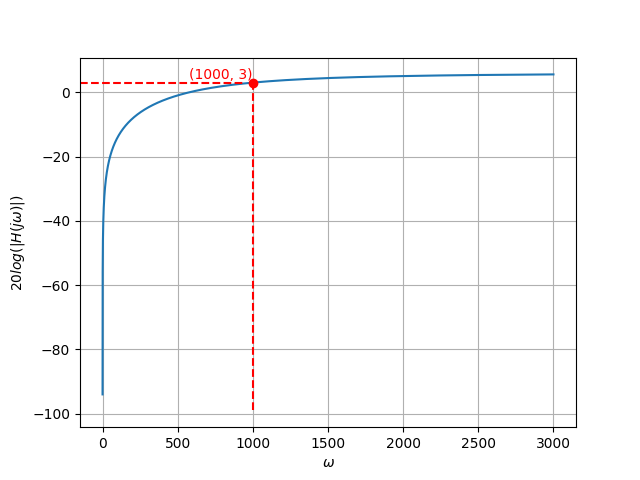
\includegraphics[width=1.0\columnwidth]{2022/EC/26/figs/plot1.png}
  \caption{\centering Frequency response plot}
  \label{fig:26fig3}
\end{figure}
%\end{document}




The system is described by the equation
\[ y(t) = x(e^{-t}). \]

The system is:
\begin{itemize}
    \item[(A)] non-linear and causal.
    \item[(B)] linear and non-causal.
    \item[(C)] non-linear and non-causal.
    \item[(D)] linear and causal.
\end{itemize}
\fi
\textbf{Solution:}\\

\textbf{Homogeneity Test:}\\
For input \(x_1(e^{-t})\), the output will be \(y_1(t)\).
\begin{align}
y_1(t) = x_1(e^{-t})
\end{align}
Multiplying both sides by a scalar quantity 'a'
\begin{align}
ay_1(t) = ax_1(e^{-t})
\end{align}
For input \(x_2(e^{-t})\), the output will be \(y_2(t)\).
\begin{align}
y_2(t) = x_2(e^{-t})
\end{align}
Multiplying both sides by a scalar quantity 'b'
\begin{align}
by_2(t) = bx_2(e^{-t})
\end{align}
Adding the above equations we get:
\begin{align}
ay_1(t) + by_2(t) = ax_1(e^{-t}) + bx_2(e^{-t})
\end{align}
Let us assume that, for input \(ax_1(e^{-t}) + bx_2(e^{-t})\), the output will be \(y_3(t)\).
\begin{align}
y_3(t) = ax_1(e^{-t}) + bx_2(e^{-t})
\end{align}
But, \(ay_1(t) + by_2(t) = ax_1(e^{-t}) + bx_2(e^{-t})\)\\
Therefore;
\begin{align}
y_3(t) = ay_1(t) + by_2(t)
\end{align}

The system satisfies homogeneity, as scaling the input scales the output.\\

\textbf{Additivity Test:}\\
From the given system;
\begin{align}
y(t) = x(e^{-t})
\end{align}
\begin{align}
y(0) = x(e^{0})
\end{align}
\begin{align}
y(1) = x(e) = x(2.71)
\end{align}
So, the present value of output depends on the future value of input, indicating non-causality.

Therefore, the correct answer is:
\textbf{(B) linear and non-causal}

%\end{document}

